% !TeX root = ../main.tex
% Add the above to each chapter to make compiling the PDF easier in some editors.

\chapter{Experimental Results and Analysis}\label{chapter:presentation_of_the_results}

\section{Reference and Query Images}

\section{Evaluation Metrics}

To appreciate the quality of the estimations, the most widely used pose error functions are the \ac{ADD} and the \ac{ADD-S} metrics, both introduced by Hinterstoisser et al. \cite{10.1007/978-3-642-37331-2_42}. For an object model $\mathcal{M}$, we compute the average distance to the corresponding model point. Therefore the error of an estimated pose $\hat{\bm{\mathrm{P}}}=(\hat{\bm{\mathrm{R}}},\,\hat{\bm{\mathrm{T}}})$ w.r.t. the ground truth pose $\bar{\bm{\mathrm{P}}}=(\bar{\bm{\mathrm{R}}},\,\bar{\bm{\mathrm{T}}})$ is calculated as follows:

\begin{align}
	\textit{\footnotemark}e_\mathrm{ADD}(\hat{\bm{\mathrm{P}}},\,\bar{\bm{\mathrm{P}}},\,\mathcal{M})&\stackrel{\text{def.}}{=}\underset{\bm{\mathrm{x}}\in\mathcal{M}}{\mathrm{avg}}\norm\bigg{\bar{\bm{\mathrm{P}}}\bm{\mathrm{x}}^\star-\hat{\bm{\mathrm{P}}}\bm{\mathrm{x}}^\star}_2 \\
	&=\underset{\bm{\mathrm{x}}\in\mathcal{M}}{\mathrm{avg}}\norm\bigg{(\bar{\bm{\mathrm{R}}}\bm{\mathrm{x}}+\bar{\bm{\mathrm{T}}})-(\hat{\bm{\mathrm{R}}}\bm{\mathrm{x}}+\hat{\bm{\mathrm{T}}})}_2
\end{align}
\footnotetext{In this context, the vector $\bm{\mathrm{x}}^\star$ represents a vector that has been extended by appending a 1, specifically for the purpose of matrix multiplication.}

When the model $\mathcal{M}$ has symmetries that leads to indistinguishable views, the error is computed as the average distance to the closest model point:
 
\begin{align}
	e_{\mathrm{ADD}\text{-}\mathrm{S}}(\hat{\bm{\mathrm{P}}},\,\bar{\bm{\mathrm{P}}},\,\mathcal{M})&\stackrel{\text{def.}}{=} \underset{\bm{\mathrm{x}}_1\in\mathcal{M}}{\mathrm{avg}}\min\limits_{\bm{\mathrm{x}}_2\in\mathcal{M}}\norm\bigg{\bar{\bm{\mathrm{P}}}\bm{\mathrm{x}}_1^\star-\hat{\bm{\mathrm{P}}}\bm{\mathrm{x}}_2^\star}_2 \\
	&=\underset{\bm{\mathrm{x}}_1\in\mathcal{M}}{\mathrm{avg}}\min\limits_{\bm{\mathrm{x}}_2\in\mathcal{M}}\norm\bigg{(\bar{\bm{\mathrm{R}}}\bm{\mathrm{x}}_1+\bar{\bm{\mathrm{T}}})-(\hat{\bm{\mathrm{R}}}\bm{\mathrm{x}}_2+\hat{\bm{\mathrm{T}}})}_2
\end{align}

It's important to point out that $e_{\mathrm{ADD}\text{-}\mathrm{S}}$ is more lenient compared to $e_\mathrm{ADD}$, and should only be applied in cases where there is a definite presence of symmetry in the object and the estimated pose is already notably precise. Otherwise, using $e_{\mathrm{ADD}\text{-}\mathrm{S}}$ becomes irrelevant since the estimation would be unfairly advantaged. In the illustrations below, we consistently provide both metrics, however it is up to the reader to assess the relevance of $e_{\mathrm{ADD}\text{-}\mathrm{S}}$ based on the observed spacecraft. 


\section{Vizualisation and Quantitative Evaluation}
\pagestyle{fancy}
\fancyhf{}
\fancyhead[C]{\small\textsc{4.3. Vizualisation and Quantitative Evaluation}}
\fancyfoot[C]{\small\thepage} % center the page number in the footer
\renewcommand{\footrulewidth}{0.4pt} % adds a line above the footer

\begin{figure}[h]
    \centering
    \begin{minipage}{0.45\linewidth}
        \centering
        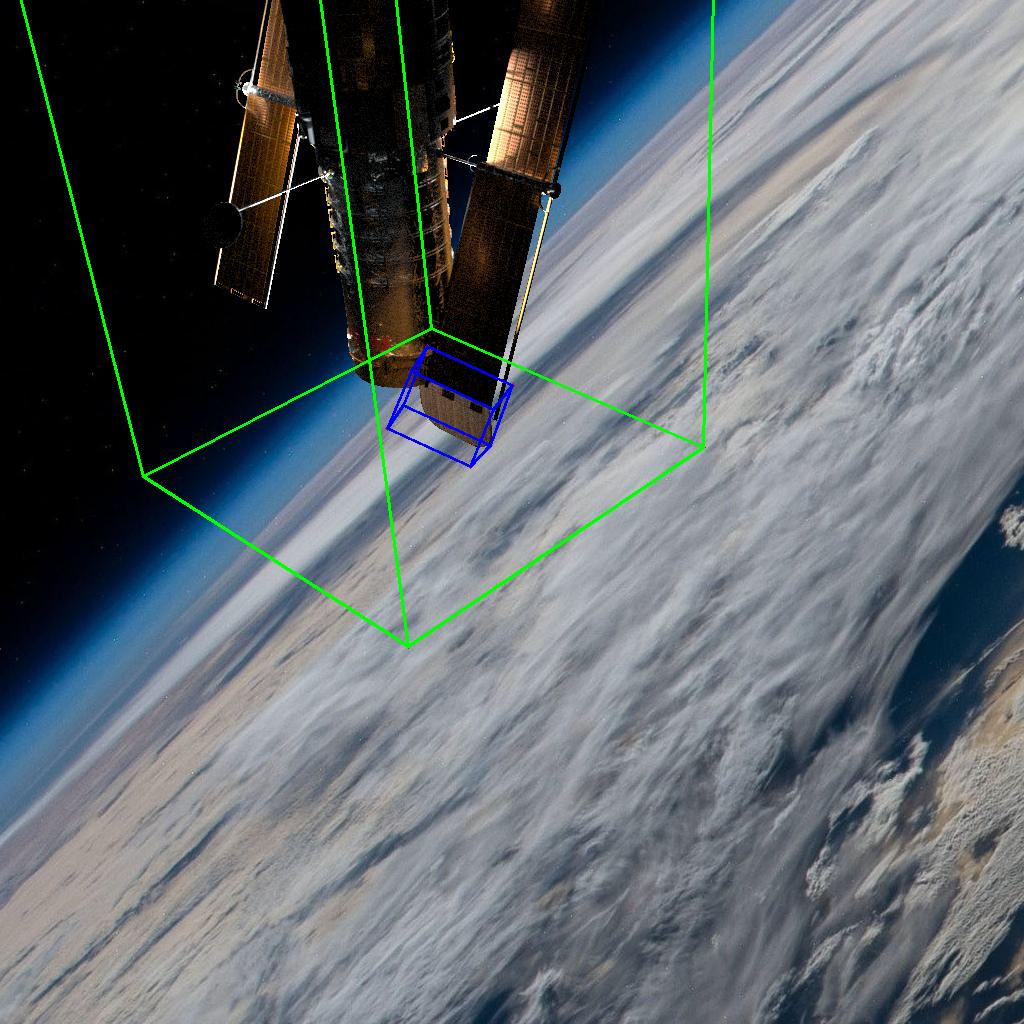
\includegraphics[width=\linewidth]{data/fig2.jpg} % First image
        \caption{Hubble Space Telescope with earth rendered background, 1024x1024 first query image}
        \label{fig:fig2}
    \end{minipage}\hfill
    \begin{minipage}{0.45\linewidth}
        \centering
        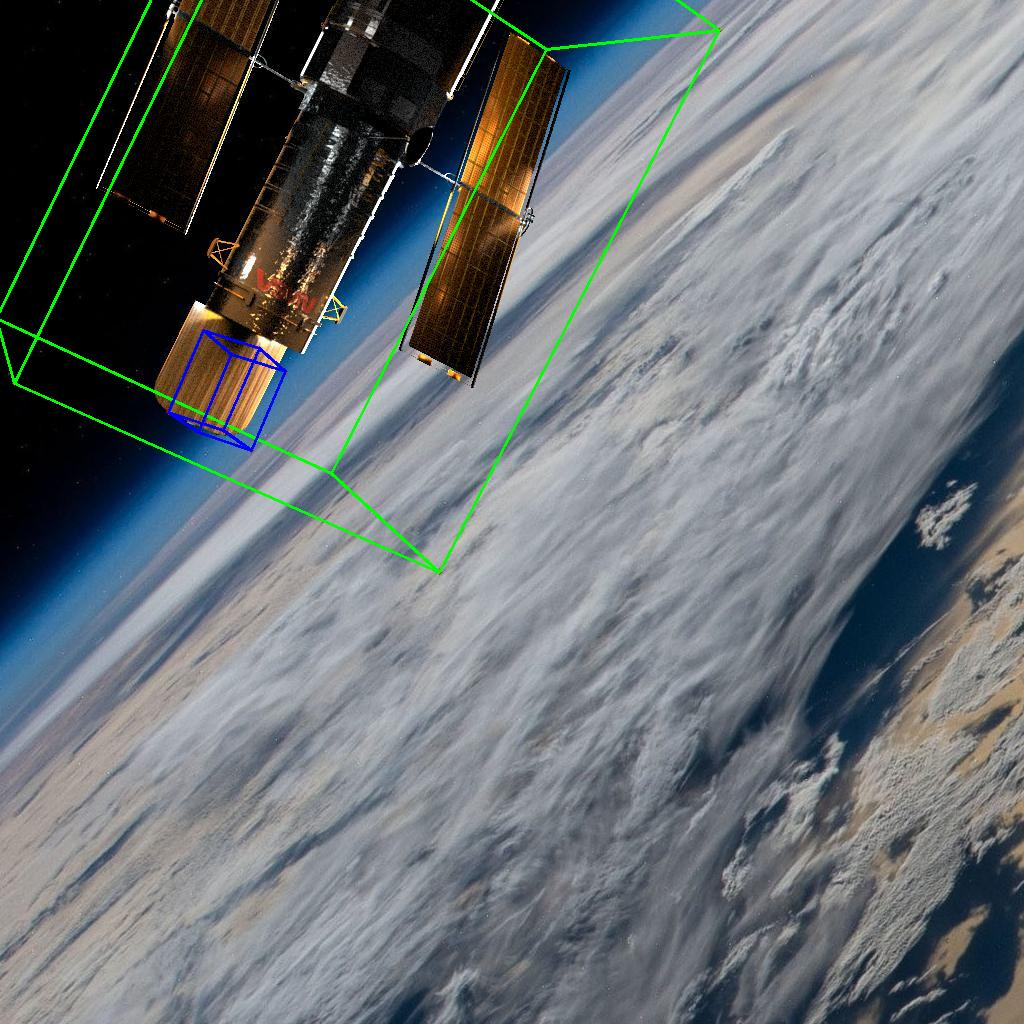
\includegraphics[width=\linewidth]{data/fig1.jpg} % Second image
        \caption{Hubble Space Telescope with earth rendered background, 1024x1024 second query image}
        \label{fig:fig1}
    \end{minipage}
\end{figure}

\begin{figure}[h]
    \centering
    \begin{minipage}{0.45\linewidth}
        \centering
        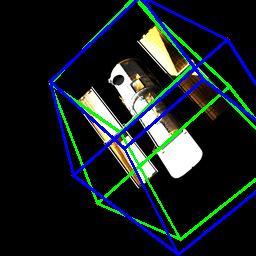
\includegraphics[width=\linewidth]{data/fig3.jpg} % First image
        \caption{Hubble Space Telescope, no background, 256x256 query image, $e_\mathrm{ADD}=2.925$, $e_{\mathrm{ADD}\text{-}\mathrm{S}}=1.183$ }
        \label{fig:fig3}
    \end{minipage}\hfill
    \begin{minipage}{0.45\linewidth}
        \centering
        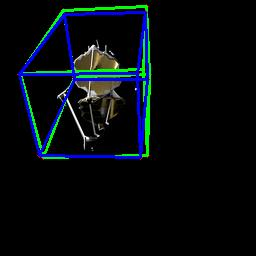
\includegraphics[width=\linewidth]{data/fig4.jpg} % Second image
        \caption{James Webb Space Telescope, no background, 256x256 query image, $e_\mathrm{ADD}=1.415$, $e_{\mathrm{ADD}\text{-}\mathrm{S}}=0.808$ }
        \label{fig:fig4}
    \end{minipage}
\end{figure}

\begin{figure}[h]
    \centering
    \begin{minipage}{0.45\linewidth}
        \centering
        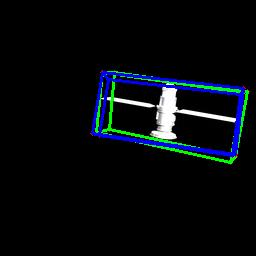
\includegraphics[width=\linewidth]{data/fig5.jpg} % First image
        \caption{Cosmos Link, no background, 256x256 query image, $e_\mathrm{ADD}=1.718$, $e_{\mathrm{ADD}\text{-}\mathrm{S}}=0.383$ }
        \label{fig:fig5}
    \end{minipage}\hfill
    \begin{minipage}{0.45\linewidth}
        \centering
        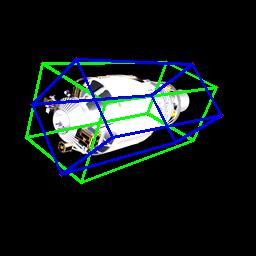
\includegraphics[width=\linewidth]{data/fig6.jpg} % Second image
        \caption{Rocket Body, no background, 256x256 query image, $e_\mathrm{ADD}=1.713$, $e_{\mathrm{ADD}\text{-}\mathrm{S}}=0.252$ }
        \label{fig:fig6}
    \end{minipage}
\end{figure}

\begin{figure}[h]
    \centering
    \begin{minipage}{0.45\linewidth}
        \centering
        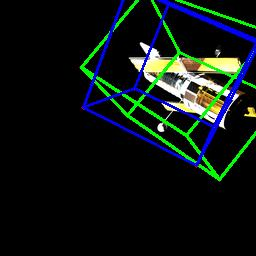
\includegraphics[width=\linewidth]{data/fig7.jpg} % First image
        \caption{Hubble Space Telescope, no background, 256x256 query image, $e_\mathrm{ADD}=6.514$, $e_{\mathrm{ADD}\text{-}\mathrm{S}}=1.571$ }
        \label{fig:fig7}
    \end{minipage}\hfill
    \begin{minipage}{0.45\linewidth}
        \centering
        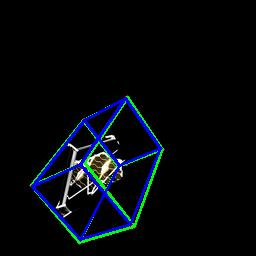
\includegraphics[width=\linewidth]{data/fig8.jpg} % Second image
        \caption{James Webb Space Telescope, no background, 256x256 query image, $e_\mathrm{ADD}=2.224$, $e_{\mathrm{ADD}\text{-}\mathrm{S}}=1.261$ }
        \label{fig:fig8}
    \end{minipage}
\end{figure}

\begin{figure}[h]
    \centering
    \begin{minipage}{0.45\linewidth}
        \centering
        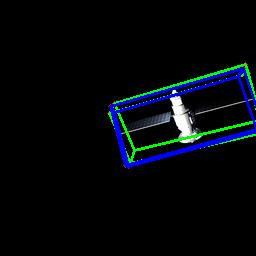
\includegraphics[width=\linewidth]{data/fig9.jpg} % First image
        \caption{Cosmos Link, no background, 256x256 query image, $e_\mathrm{ADD}=1.925$, $e_{\mathrm{ADD}\text{-}\mathrm{S}}=0.377$ }
        \label{fig:fig9}
    \end{minipage}\hfill
    \begin{minipage}{0.45\linewidth}
        \centering
        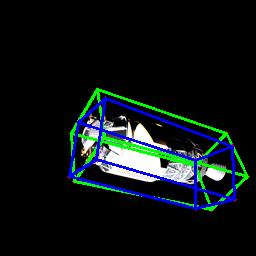
\includegraphics[width=\linewidth]{data/fig10.jpg} % Second image
        \caption{Rocket Body, no background, 256x256 query image, $e_\mathrm{ADD}=1.982$, $e_{\mathrm{ADD}\text{-}\mathrm{S}}=0.501$ }
        \label{fig:fig10}
    \end{minipage}
\end{figure}

\begin{figure}[ht]
  \centering
  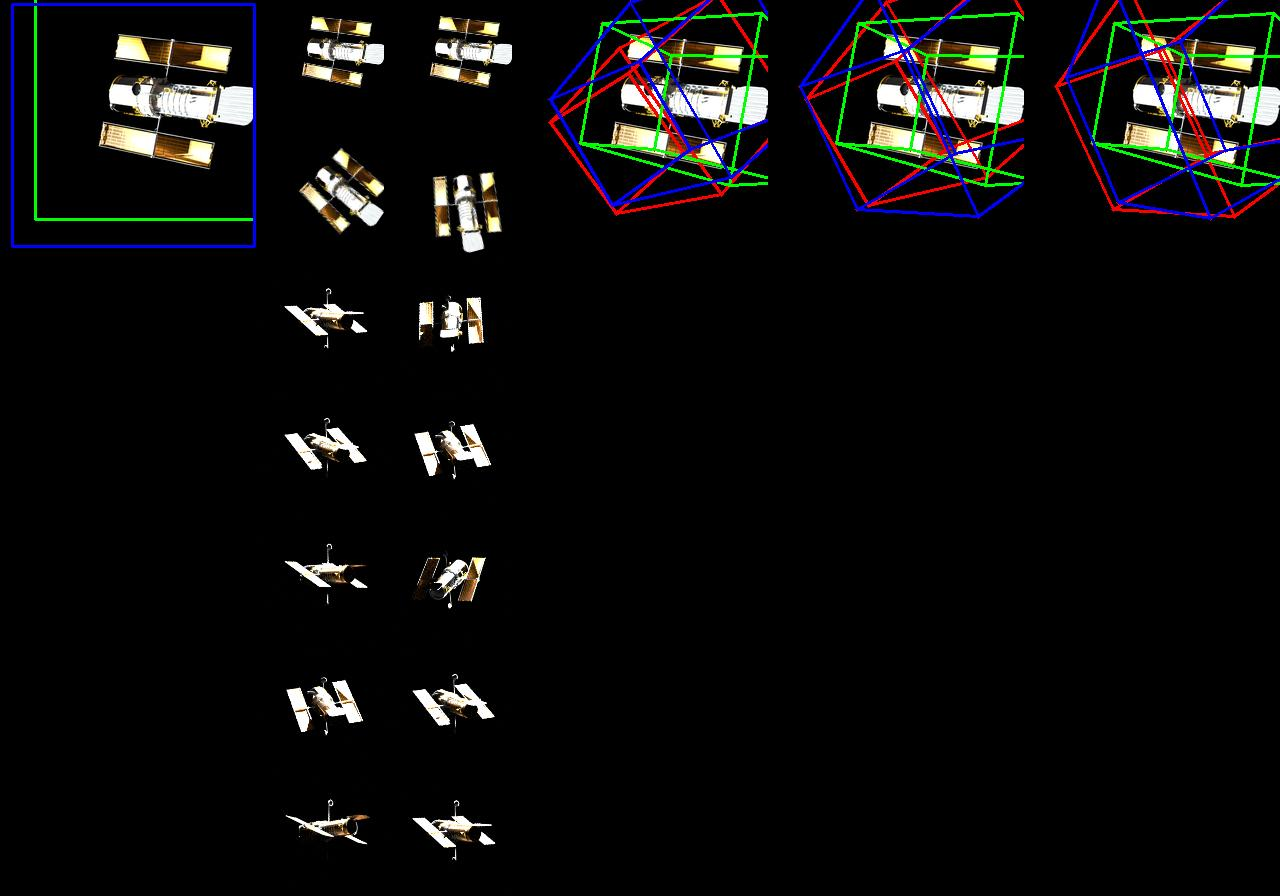
\includegraphics[width=\textwidth]{data/fig11.jpg}
  \caption{Hubble Space Telescope, no background, intermediary result, $e_\mathrm{ADD}=9.577$, $e_{\mathrm{ADD}\text{-}\mathrm{S}}=5.196$}
  \label{fig:fig11}
\end{figure}

\begin{figure}[ht]
  \centering
  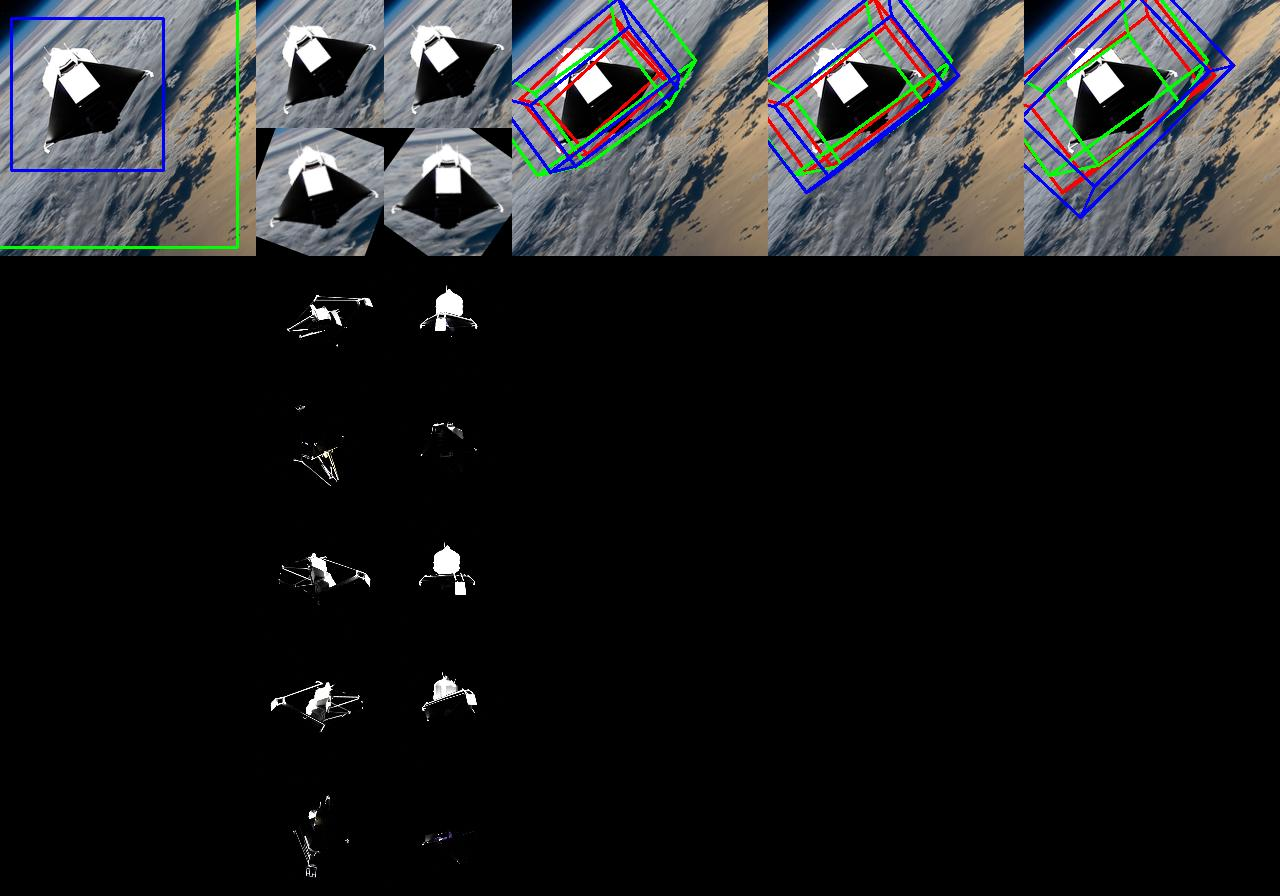
\includegraphics[width=\textwidth]{data/fig12.jpg}
  \caption{James Webb Space Telescope, with earth rendered background, intermediary result, $e_\mathrm{ADD}=10.934$, $e_{\mathrm{ADD}\text{-}\mathrm{S}}=4.317$}
  \label{fig:fig12}
\end{figure}

\begin{figure}[ht]
  \centering
  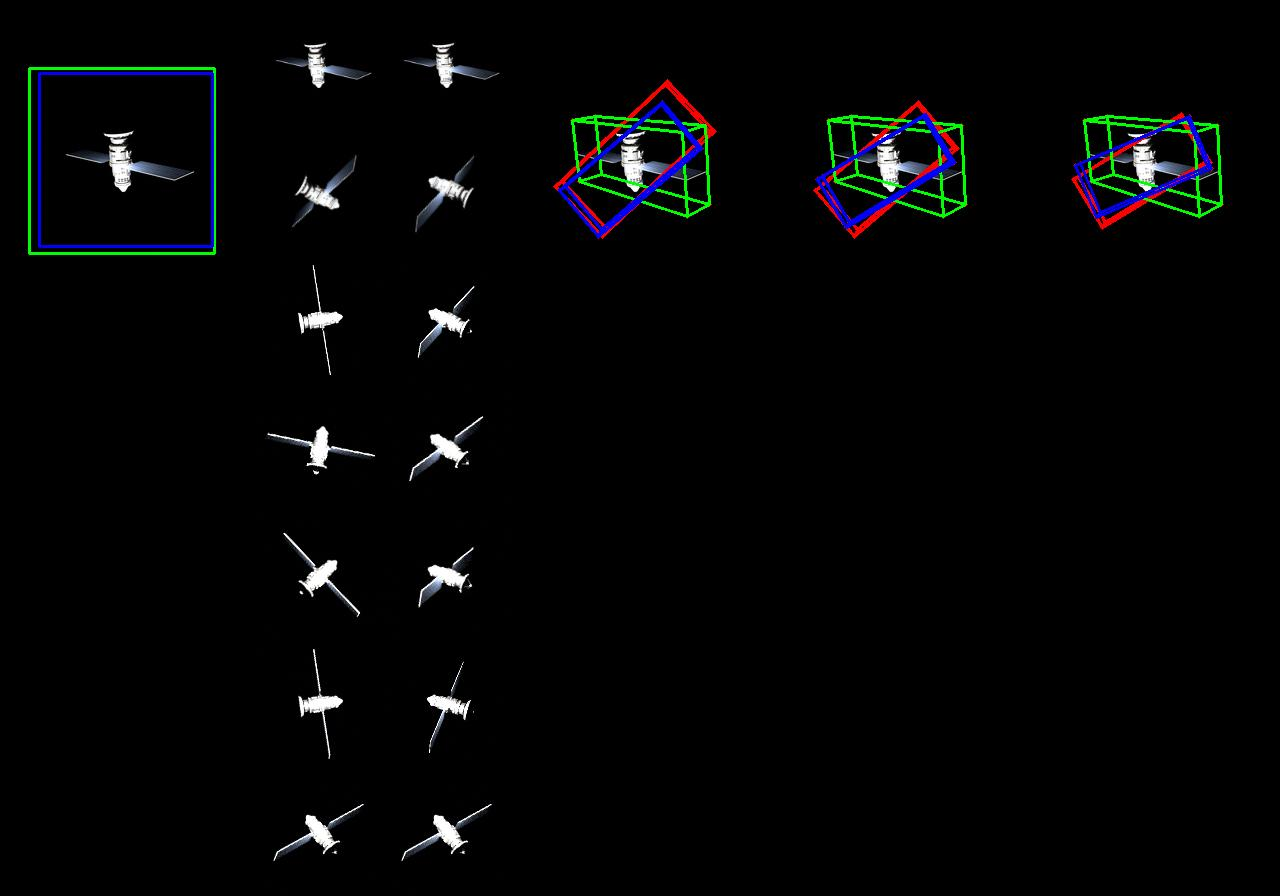
\includegraphics[width=\textwidth]{data/fig13.jpg}
  \caption{Cosmos Link, no background, intermediary result, $e_\mathrm{ADD}=11.094$, $e_{\mathrm{ADD}\text{-}\mathrm{S}}=6.127$}
  \label{fig:fig13}
\end{figure}

\begin{figure}[ht]
  \centering
  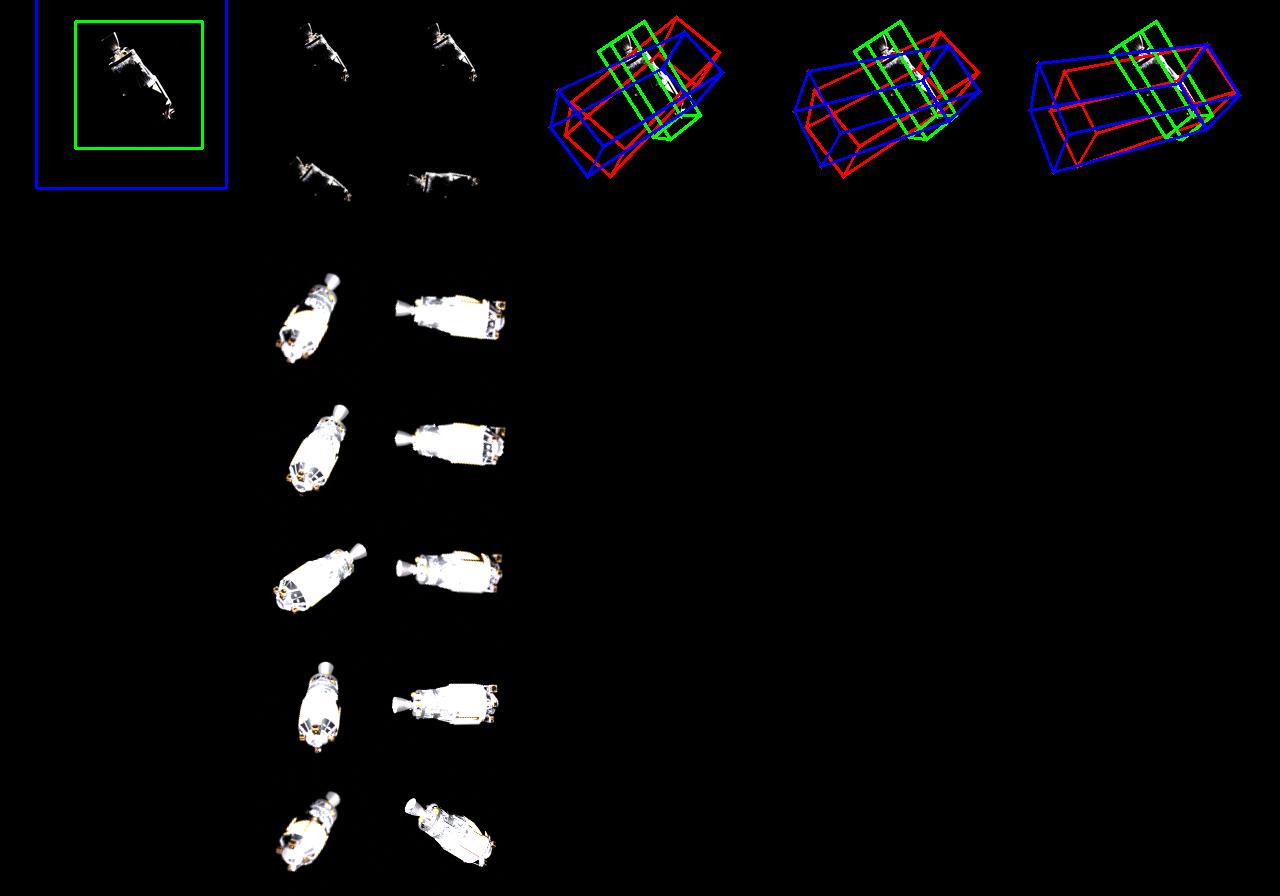
\includegraphics[width=\textwidth]{data/fig14.jpg}
  \caption{Rocket Body, no background, intermediary result, $e_\mathrm{ADD}=29.335$, $e_{\mathrm{ADD}\text{-}\mathrm{S}}=17.743$}
  \label{fig:fig14}
\end{figure}

\begin{figure}[ht]
  \centering
  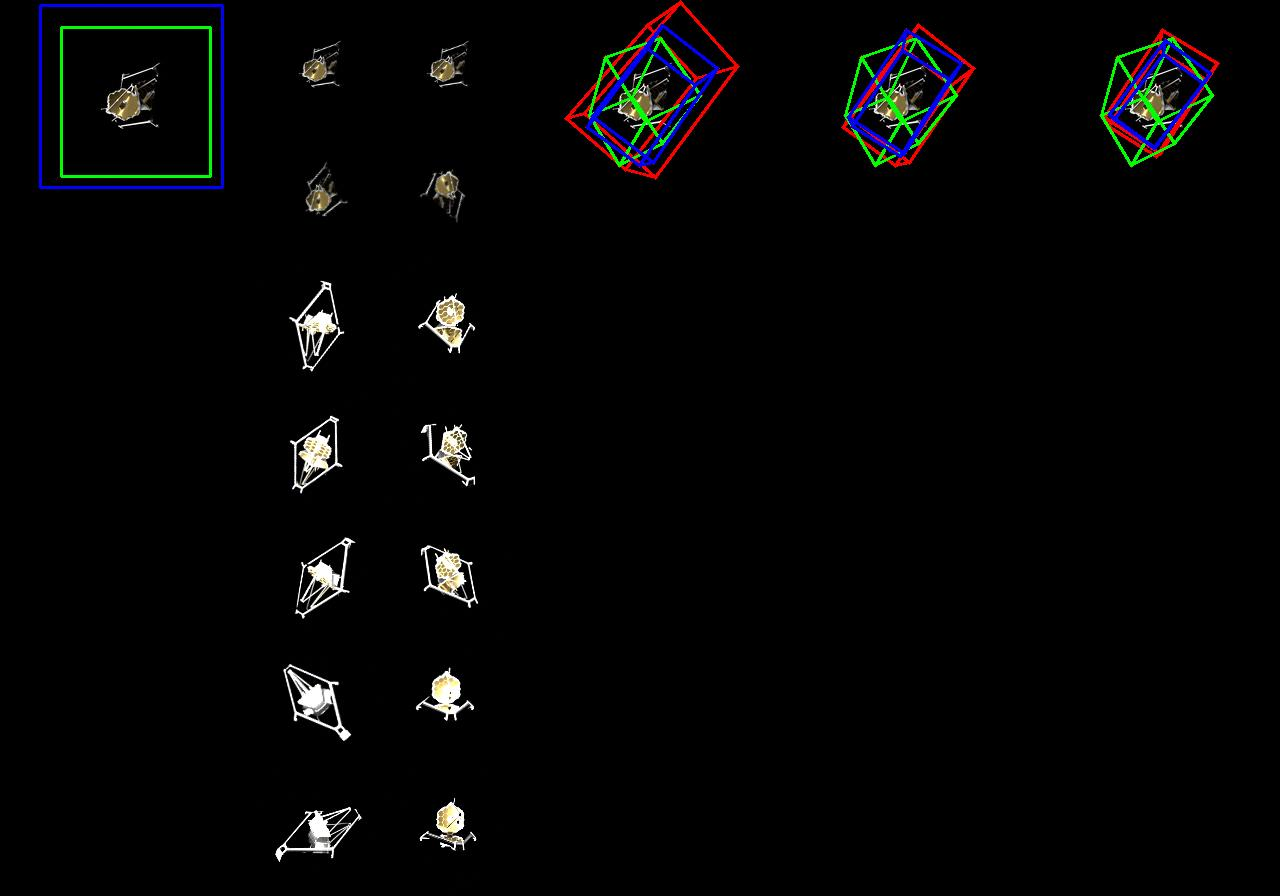
\includegraphics[width=\textwidth]{data/fig15.jpg}
  \caption{James Webb Space Telescope, with no background, intermediary result, $e_\mathrm{ADD}=21.983$, $e_{\mathrm{ADD}\text{-}\mathrm{S}}=12.358$}
  \label{fig:fig15}
\end{figure}

\begin{figure}[ht]
  \centering
  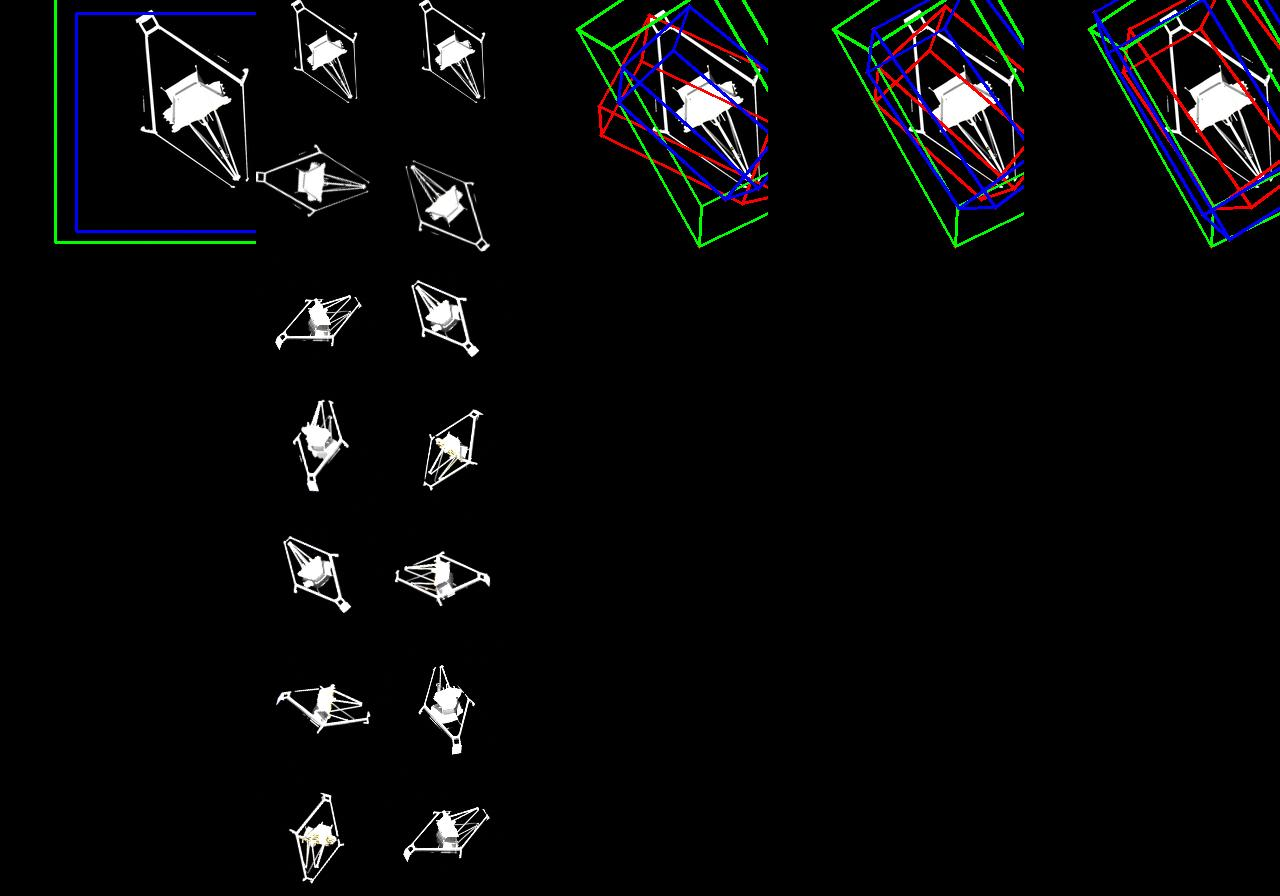
\includegraphics[width=\textwidth]{data/fig16.jpg}
  \caption{James Webb Space Telescope, with no background, intermediary result, $e_\mathrm{ADD}=1.060$, $e_{\mathrm{ADD}\text{-}\mathrm{S}}=0.556$}
  \label{fig:fig16}
\end{figure}

